%\documentclass[]{scrartcl}
\documentclass[]{article}
% sans-serif font
\renewcommand{\familydefault}{\sfdefault}
% Bibtex citations
\usepackage{cite}
% sequence diagrams
\usepackage{pgf-umlsd}
% one inch margins
\usepackage[a4paper, margin=1in]{geometry}

\usepackage{tikz}
\usetikzlibrary{decorations.pathreplacing,angles,quotes}

\title{Minecraft: Ray Traced}
%\subtitle{Or: A dynamic acceleration structure for voxel worlds}
\author{Marco Jonkers}

\begin{document}

\maketitle

\begin{abstract}
This project attempts to implement a GPU ray tracer in the video game Minecraft, using CUDA.
The ray tracing itself is done in CUDA. At first, I attempt to ray trace the vertex buffers given by Minecraft. Then, I implement my own data structures for increased performance.
\end{abstract}

\section{Goal}
Similar to other ray tracing research projects by Intel Corporation.
Also shortly explain the benefits of ray tracing versus regular rasterization.
Minecraft's world is made up of voxels, which is nice for ray tracing.

\section{Setup}
Here I explain how the project is set up and the technologies involved.
Minecraft is coded in Java.
The Minecraft Forge project allows me to do two things:
  Listen to specific events using pre-installed hooks
  Edit Minecraft bytecode before it is loaded
Using Java Native Interface (JNI), I can call into C++ code from Java.
The C++ code contains the CUDA kernel.
Data is passed between OpenGL and CUDA using CUDA's graphics interop layer.

\section{Minecraft Rendering System}
There are four geometry groups:
\begin{description}
  \item[Solid] This is solid geometry.
  \item[Cutout] Used for glass.
  \item[Mipped Cutout] Identical to Cutout, but mipmapped.
  \item[Translucent] Used for block which have partial transparency (alpha blending).
\end{description}
Every geometry group has its own vertex buffer.

\section{Raytracing Minecraft's Vertex Buffers Directly}

I explain something here that is found in Figure ~\ref{fig:sequence}.

\section{Challenges}
The challenges of this project include:
\begin{description}
  \item [Ray tracing performance] Because of gameplay.
  \item [Acceleration structure rebuild speed] Because of gameplay.
\end{description}

\section{Static Geometry}
Test for citing \cite{amanatides1987fast}.

I am also citing \cite{ivson2009gpu}.

I am also citing \cite{reinhard2000dynamic}.

\section{Dynamic Geometry}
This section describes ray tracing dynamic objects, such as NPCs.

\section{Benchmarks}


\section{Future work}
Future work is addressed here.

\bibliography{minecraft_ray_traced}{}
\bibliographystyle{apalike}

\listoffigures

% Code flow structure
\begin{figure}
  \centering
  \begin{sequencediagram}
    \newthread{minecraft}{Forge Minecraft}{}
    \newinst[2]{forge}{Forge Mod}{}
    \newinst[2]{loader}{C++/CUDA}{}
    \begin{call}{minecraft}{transform()}{forge}{}
    \end{call}
    \postlevel
    \begin{call}{minecraft}{Raytracer()}{forge}{}
      \begin{call}{forge}{init()}{loader}{}
      \end{call}
    \end{call}
    %    \postlevel
    %    \begin{call}{minecraft}{onPreInitGuiEvent()}{forge}{}
    %      \begin{call}{forge}{resize()}{loader}{}
    %      \end{call}
    %    \end{call}
    \begin{sdblock}{Main Loop}{}
      \begin{call}{minecraft}{initialize()}{forge}{}
        \begin{call}{forge}{setViewEntity()}{loader}{}
        \end{call}
      \end{call}
      \postlevel
      \begin{call}{minecraft}{addRenderChunk()}{forge}{}
      \end{call}
      \postlevel
      \begin{call}{minecraft}{renderChunkLayer()}{forge}{}
        \begin{call}{forge}{setVertexBuffer()}{loader}{}
          \begin{call}{loader}{GetIntField()}{loader}{glBufferId}
          \end{call}
        \end{call}
      \end{call}
      \postlevel
      \begin{call}{minecraft}{renderWorld()}{forge}{}
        \begin{call}{forge}{setViewingPlane()}{loader}{}
        \end{call}
        \postlevel
        \begin{call}{forge}{raytrace()}{loader}{texture ID}
          \begin{call}{loader}{Kernel()}{loader}{}
          \end{call}
        \end{call}
      \end{call}
    \end{sdblock}
  \end{sequencediagram}
  \caption[Sequence diagram]{Sequence diagram showing interaction between the modules}
  \label{fig:sequence}
\end{figure}

\begin{figure}
  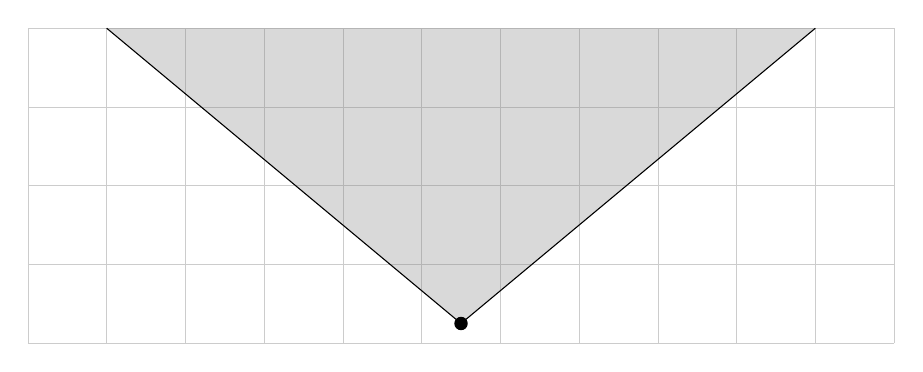
\begin{tikzpicture}
  \draw[step=1cm,very thin,opacity=0.2] (-5, 0) grid (6, 4);
  % hfov = 102.4478577779882556443232935315
  \fill[color=gray,opacity=0.3] (0.5, 0.25) -- (-4.0,4.0) -- (5.0,4.0) -- (0.5,0.25);
  \draw (0.5,0.25) -- (-4.0,4.0);
  \draw (0.5,0.25) -- (5.0,4.0);
  \draw[fill] (0.5,0.25) circle (.5ex);
  %\draw[very thick,->] (0.5,0.25) -- ++(141.22392888899412782216164676575:6cm);
  %\draw[very thick,->] (0.5,0.25) -- ++(38.77607111100587217783835323425:6cm);
  %\draw[very thick,->] (0.5,0.25) -- (0.5,4.0);
  \end{tikzpicture}
  \centering
  \caption[Player's field of view]{A player's default field of view, facing north. Diagonal rays traverse more cells.}
\end{figure}

\begin{figure}
  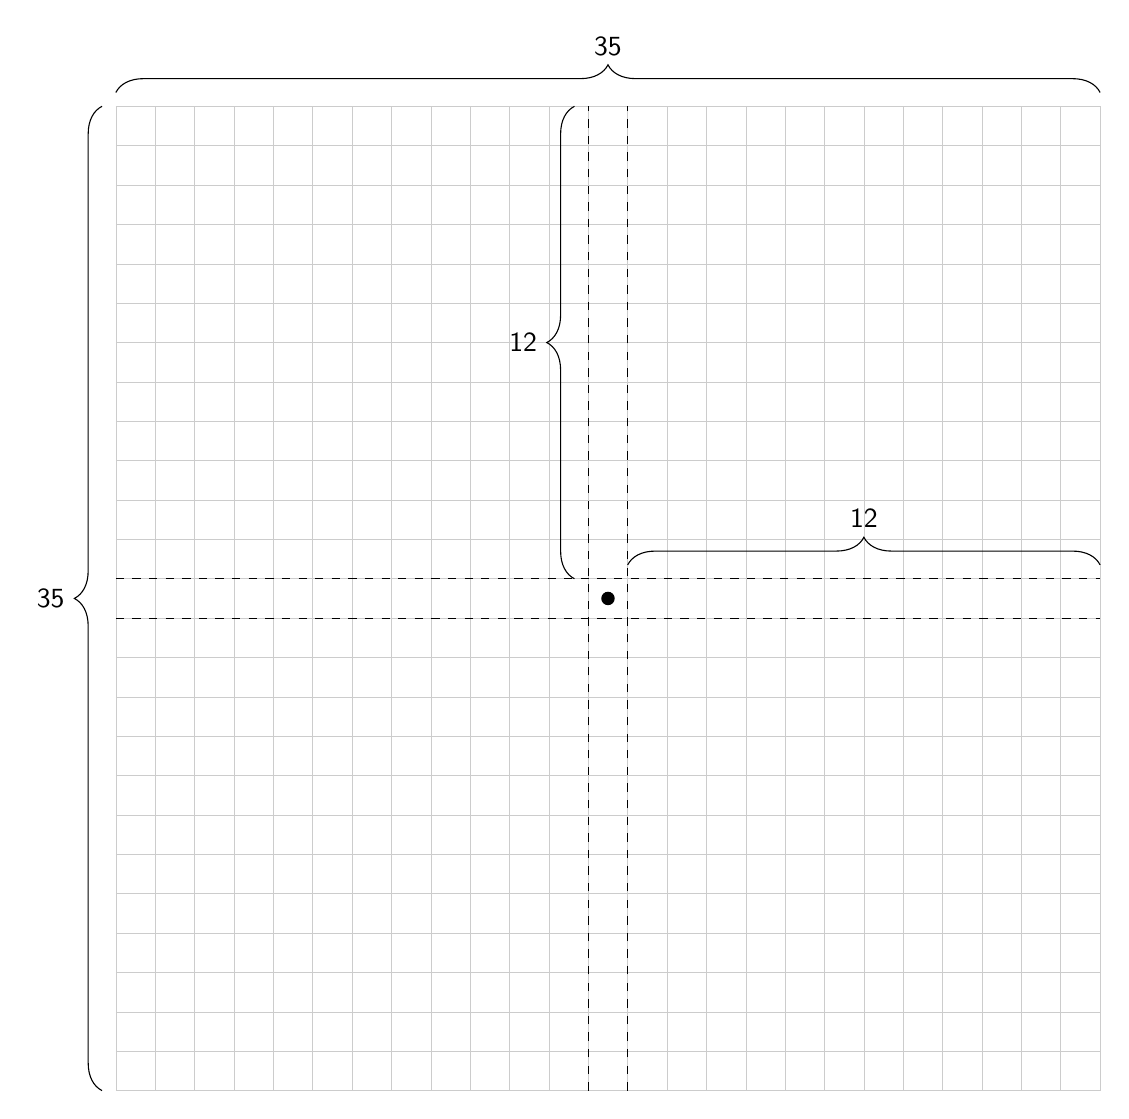
\begin{tikzpicture}
  \draw[step=0.5cm,very thin,opacity=0.2] (-6,-6) grid (6.5,6.5);
  %\fill (0,0) -- (0.5,0) -- (0.5,0.5) -- (0,0.5) -- (0,0);
  \draw[dashed] (-6,0) -- (6.5,0);
  \draw[dashed] (-6,0.5) -- (6.5,0.5);
  \draw[dashed] (0,-6) -- (0,6.5);
  \draw[dashed] (0.5,-6) -- (0.5,6.5);
  \draw[decoration={brace,amplitude=10pt,raise=5pt},decorate] (0.5,0.5) -- node[above=15pt] {12} (6.5,0.5);
  \draw[decoration={brace,amplitude=10pt,raise=5pt},decorate] (0,0.5) -- node[left=15pt] {12} (0,6.5);
  \draw[decoration={brace,amplitude=10pt,raise=5pt},decorate] (-6,6.5) -- node[above=15pt] {35} (6.5,6.5);
  \draw[decoration={brace,amplitude=10pt,raise=5pt},decorate] (-6,-6) -- node[left=15pt] {35} (-6,6.5);
  \draw[fill] (0.25,0.25) circle (.5ex);
  %\draw[decoration={brace,mirror,raise=5pt},decorate] (0.5,0) -- node[below=6pt] {Render distance} (6.5,0);
  \end{tikzpicture}
  \centering
  \caption[2D View of vertex buffer array]{A two-dimensional view of the vertex buffer array, assuming a render distance of 12. Each cell contains 16 RenderChunks.}
\end{figure}

\begin{figure}
  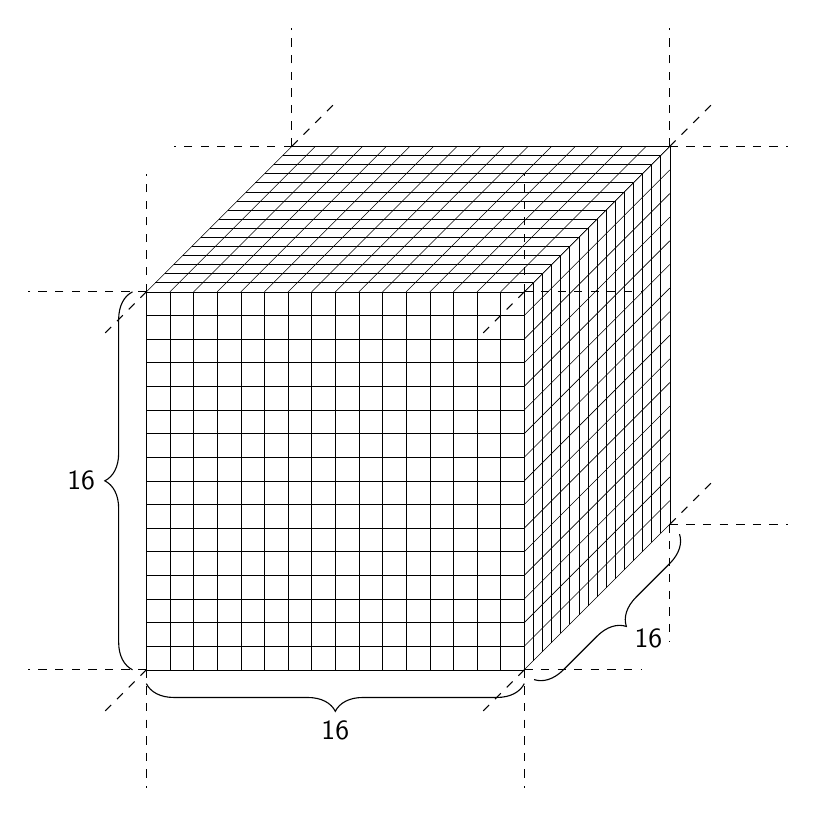
\begin{tikzpicture}[scale=0.3]
  \foreach \x in{0,...,16} {
    \draw[very thin] (0,\x ,16) -- (16,\x ,16);
    \draw[very thin] (\x ,0,16) -- (\x ,16,16);
    \draw[very thin] (16,\x ,16) -- (16,\x ,0);
    \draw[very thin] (\x ,16,16) -- (\x ,16,0);
    \draw[very thin] (16,0,\x ) -- (16,16,\x );
    \draw[very thin] (0,16,\x ) -- (16,16,\x );
  }
  % right
  \draw[dashed] (16,0,0) -- ++(5,0,0);
  \draw[dashed] (16,16,0) -- ++(5,0,0);
  \draw[dashed] (16,16,16) -- ++(5,0,0);
  \draw[dashed] (16,0,16) -- ++(5,0,0);
  % top
  \draw[dashed] (0,16,0) -- ++(0,5,0);
  \draw[dashed] (16,16,0) -- ++(0,5,0);
  \draw[dashed] (16,16,16) -- ++(0,5,0);
  \draw[dashed] (0,16,16) -- ++(0,5,0);
  % back
  \draw[dashed] (0,16,0) -- ++(0,0,-5);
  \draw[dashed] (16,16,0) -- ++(0,0,-5);
  \draw[dashed] (16,0,0) -- ++(0,0,-5);
  % front
  \draw[dashed] (0,16,16) -- ++(0,0,5);
  \draw[dashed] (16,16,16) -- ++(0,0,5);
  \draw[dashed] (16,0,16) -- ++(0,0,5);
  \draw[dashed] (0,0,16) -- ++(0,0,5);
  % left
  \draw[dashed] (0,0,16) -- ++(-5,0,0);
  \draw[dashed] (0,16,16) -- ++(-5,0,0);
  \draw[dashed] (0,16,0) -- ++(-5,0,0);
  % bottom
  \draw[dashed] (16,0,0) -- ++(0,-5,0);
  \draw[dashed] (16,0,16) -- ++(0,-5,0);
  \draw[dashed] (0,0,16) -- ++(0,-5,0);
  % curly braces
  \draw[decoration={brace,amplitude=10pt,raise=5pt},decorate] (0,0,16) -- node[left=15pt]{16} (0,16,16);
  \draw[decoration={brace,mirror,amplitude=10pt,raise=5pt},decorate] (0,0,16) -- node[below=15pt]{16} (16,0,16);
  \draw[decoration={brace,mirror,amplitude=10pt,raise=5pt},decorate] (16,0,16) -- node[below=15pt,right=10pt]{16} (16,0,0);
  \end{tikzpicture}
  \centering
  \caption[Diagram of a RenderChunk]{A single, completely filled RenderChunk.}
\end{figure}

\end{document}
